\documentclass{article}
\usepackage{amsmath}
\usepackage[margin=0.5in]{geometry}
\usepackage{amssymb}
\usepackage{parskip}
\usepackage{tikz}
\usepackage{siunitx}
\usepackage{circuitikz}
\usetikzlibrary{patterns}
\usetikzlibrary{arrows.meta, decorations.pathmorphing}

% Define colors
\definecolor{bluecolor}{RGB}{173,216,230} % Light blue
\definecolor{purplecolor}{RGB}{210,180,222} % Light purple
\definecolor{pinkcolor}{RGB}{255,182,193} % Light pink
\definecolor{orangecolor}{RGB}{252, 213, 180} % Light orange

\title{EMCH 354 FINAL EXAM Solutions}
\author{Jacob Vaught}
\date{04-30-2024}

\begin{document}
\maketitle

Thanks for a great Semester! 

\section{Problem \#1 [15 pt]}
\subsection{Problem 1.1}
Given the temperature difference in Celsius:
\[ \Delta T_{\text{C}} = 50^{\circ}C \]

To convert this to Fahrenheit, use the conversion formula for temperature differences:
\[ \Delta T_{\text{F}} = \Delta T_{\text{C}} \times \frac{9}{5} \]

Substitute the given value:
\[ \Delta T_{\text{F}} = 50 \times \frac{9}{5} = 90^{\circ}F \]

Thus, the temperature difference is:
\[ \Delta T_{\text{F}} = 90^{\circ}F \]


\subsection{Problem 1.2}
Given the following options, identify which function correctly represents 1-dimensional transient conduction processes, where \( T \) is temperature, \( t \) is time, and \( x, y, z \) represent spatial dimensions:

\begin{itemize}
    \item[(a)] \( T = f(x, y, z) \) % This is incorrect as it involves three spatial dimensions.
    \item[(b)] \( T = f(x, t) \) % Correct: involves one spatial dimension and time.
    \item[(c)] \( T = f(t) \) % This suggests a purely temporal change, not spatial.
    \item[(d)] \( T = f(x, z) \) % This involves two spatial dimensions and no temporal component.
\end{itemize}

\textbf{Answer:} The correct function that represents 1-dimensional transient conduction processes is:

\[ T = f(x, t) \]

This function correctly incorporates changes in temperature over time and along one spatial dimension, which is characteristic of 1-D transient conduction.


\subsection{Problem 1.3}
The hydraulic diameter (\(D_h\)) of an annulus formed by two concentric cylinders can be calculated using the formula:

\[
D_h = \frac{4 \times \text{Area}}{\text{Wetted Perimeter}}
\]

Where the area (\(A\)) of the annulus is the difference between the area of the outer and inner circles:

\[
A = \pi \left( \frac{D_o}{2} \right)^2 - \pi \left( \frac{D_i}{2} \right)^2 = \pi \left( \frac{D_o^2 - D_i^2}{4} \right)
\]

The wetted perimeter (\(P\)) is the sum of the circumferences of the inner and outer cylinders:

\[
P = \pi D_o + \pi D_i = \pi (D_o + D_i)
\]

Substituting these values into the formula for hydraulic diameter gives:

\[
D_h = \frac{4 \times \left( \pi \frac{D_o^2 - D_i^2}{4} \right)}{\pi (D_o + D_i)}
\]

Simplifying, we obtain:

\[
D_h = \frac{D_o^2 - D_i^2}{D_o + D_i}
\]

This expression gives the hydraulic diameter of an annulus in terms of the outer diameter (\(D_o\)) and the inner diameter (\(D_i\)).

\subsection{Problem 1.4}
\textbf{* I was unsure what each arrow referred to, so I tried to list all heat transfer modes}

The dominant heat transfer modes for the processes indicated by arrows are:
\begin{itemize}
    \item \textbf{Radiation from the fire to a person or the surrounding air:} The fire emits infrared radiation that can heat objects or people nearby as well as the surrounding air, without requiring direct contact or a medium.
    
    \item \textbf{Radiation to the pot from the fire:} The pot absorbs infrared radiation from the fire, heating it up through a process that does not involve direct contact or a transferring medium.
    
    \item \textbf{Pot to water:} The heat transfer from the pot to the water inside it occurs predominantly through conduction, where heat moves from the hotter material of the pot to the cooler water through direct contact.
    
    \item \textbf{Water to air:} Heat transfer from the water to the air above it is via convection, with the movement of steam and warm air upwards indicating this process.
    
    \item \textbf{Pot to pot handle:} Heat moves along the material of the pot to its handle through conduction, given the direct physical connection and the handle's increase in temperature.
    
    \item \textbf{Pot handle to air:} The heat transfer from the pot handle to the air occurs through both convection, as warm air rises and is replaced by cooler air, and radiation, as the handle emits infrared radiation.
    
    \item \textbf{Pot handle to hand:} When a person touches the pot handle, heat is transferred to the person's hand through conduction due to the temperature difference between the hotter handle and the cooler hand.
\end{itemize}


\newpage
\section{Problem \#2 [10 pt]}
Given a duct with a rectangular cross-section \( a \times b \), and the fluid properties such as density \( \rho \), and kinematic viscosity \( \nu \), calculate the hydraulic diameter \( D_h \), average velocity \( V \), mass flux \( G \), Reynolds number \( Re \), and the friction factor \( f \) under the condition \( f \cdot Re = C \).
\subsubsection*{a) Hydraulic Diameter, \( D_h \)}
The hydraulic diameter for a duct of rectangular cross-section is given by:
\[ D_h = \frac{4 \times \text{Area}}{\text{Wetted Perimeter}} = \frac{4ab}{2(a + b)} = \frac{2ab}{a + b} \]

\subsubsection*{b) Average Velocity, \( V \)}
Using the mass flow rate \( \dot{m} \), the average velocity \( V \) can be calculated by:
\[ V = \frac{Q}{\text{Area}} = \frac{\dot{m}}{\rho ab} \]
where the volumetric flow rate \( Q = \frac{\dot{m}}{\rho} \).

\subsubsection*{c) Mass Flux, \( G \)}
Mass flux \( G \) is defined as the mass flow rate per unit area:
\[ G = \frac{\dot{m}}{ab} \]

\subsubsection*{d) Reynolds Number, \( Re \)}
The Reynolds number is calculated by:
\[ Re = \frac{V \times D_h}{\nu} \]
\[ Re = \frac{\left(\frac{\dot{m}}{\rho ab}\right) \times \left(\frac{2ab}{a + b}\right)}{\nu} \]
Simplifying this:
\[ Re = \frac{2 \dot{m}}{\rho \nu (a + b)} \]

\subsubsection*{e) Friction Factor, \( f \)}
Given the relationship \( f \cdot Re = C \), the friction factor \( f \) is simplified to:
\[ f = \frac{C}{Re} \]
This provides a straightforward method to determine \( f \) from the Reynolds number and a known constant \( C \).


\newpage
\section{Problem \#3 [10 pt]}
Consider a composite wall with equal thicknesses of concrete and brick sections. The tasks are as follows:
\begin{enumerate}
    \item[(a)] Determine the temperatures \( T_1 \) and \( T_2 \).
    \item[(b)] Calculate the percentage of the heat transfer rate, \( q \), that flows through the brick section.
\end{enumerate}
For this analysis, approximate the heat flow as one-dimensional and assume the cross-sectional area of the composite wall is \( 2 \, \text{m}^2 \). Begin by drawing the thermal circuit for the wall and identifying all four resistances.

% Insert your TikZ diagram here
\begin{center}
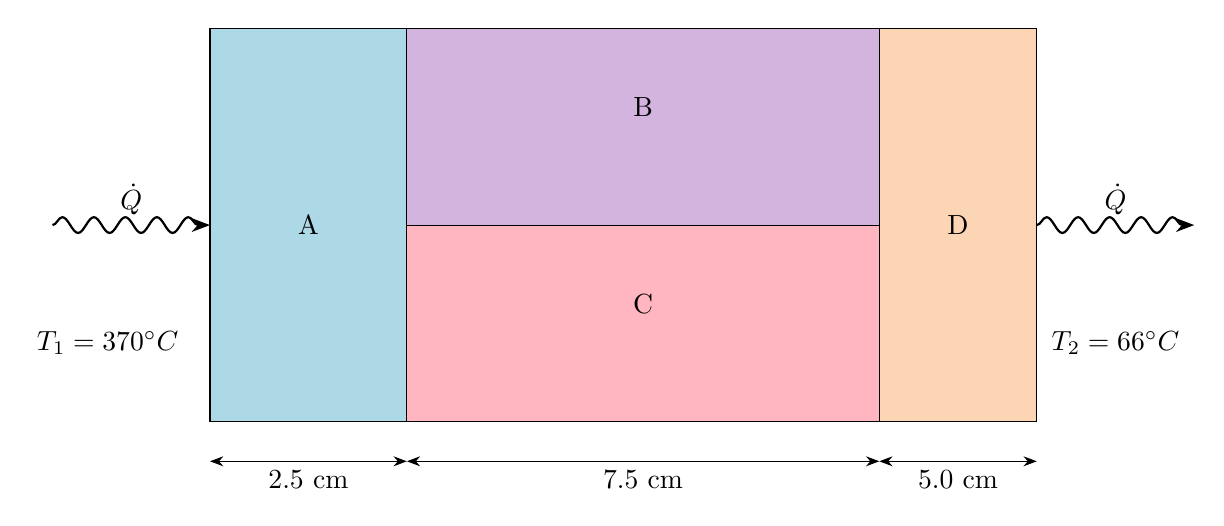
\begin{tikzpicture}[scale=0.5, >=Stealth]
% Define nodes for the temperatures
\node (T1) at (-2.6,2) {\(T_1 = 370^\circ C\)};
\node (T2) at (23,2) {\(T_2 = 66^\circ C\)};

% Draw the composite wall
\draw[fill=bluecolor] (0,0) rectangle (5,10); % Material A
\draw[fill=purplecolor] (5,5) rectangle (17,10); % Material B
\draw[fill=pinkcolor] (5,0) rectangle (17,5); % Material C
\draw[fill=orangecolor] (17,0) rectangle (21,10); % Material D

% Labels for materials
\node at (2.5,5) {A};
\node at (11,8) {B};
\node at (11,3) {C};
\node at (19,5) {D};

% Dimensions
\draw[<->] (0,-1) -- node[below] {2.5 cm} (5,-1);
\draw[<->] (5,-1) -- node[below] {7.5 cm} (17,-1);
\draw[<->] (17,-1) -- node[below] {5.0 cm} (21,-1);

% Heat flow arrows
\draw[->, thick, decorate, decoration={snake, amplitude=1mm, segment length=4mm, post length=1mm}] (-4,5) -- (0,5) node[midway,above] {\(\dot{Q}\)};
\draw[->, thick, decorate, decoration={snake, amplitude=1mm, segment length=4mm, post length=1mm}] (21,5) -- (25,5) node[midway,above] {\(\dot{Q}\)};
\end{tikzpicture}
\end{center}

\begin{center}
\begin{circuitikz}[american resistors, thick]
\tikzstyle{every node}=[font=\large]
% Defining the thermal resistances
\draw (0,-1) to[R, l=$A$, -*] (3,-1) 
      (3,0) to[short] (3,-2)
      (3,-2) to[R, l=$B$, -] (7,-2)
      (3,0) to[R, l=$C$, -] (7,0)
      (7,0) to[short] (7,-2)
      (7,-1) to[R, l=$D$, *-] (10,-1);

% Adding the input and output labels
\node at (-0.8,-1) {Input};
\node at (11,-1) {Output};
\end{circuitikz}
\end{center}

\subsection*{Solution}
The thermal resistance for each material layer is given by the formula:
\[ R = \frac{L}{kA} \]
\noindent
For the given materials, we have:

\begin{itemize}
    \item Material A: \( k_A = 0.11 \, \text{W/(m}\cdot\text{K)} \), \( L_A = 0.025 \, \text{m} \), \( A_A = 2 \, \text{m}^2 \)
    \item Material B: \( k_B = 0.76 \, \text{W/(m}\cdot\text{K)} \), \( L_B = 0.075 \, \text{m} \), \( A_B = 1 \, \text{m}^2 \)
    \item Material C: \( k_C = 0.69 \, \text{W/(m}\cdot\text{K)} \), \( L_C = 0.075 \, \text{m} \), \( A_C = 1 \, \text{m}^2 \)
    \item Material D: \( k_D = 0.147 \, \text{W/(m}\cdot\text{K)} \), \( L_D = 0.05 \, \text{m} \), \( A_D = 2 \, \text{m}^2 \)
\end{itemize}
\noindent
Using the above formula, we calculate the thermal resistance for each material:

\begin{align*}
R_A &= \frac{0.025 \, \text{m}}{0.11 \, \text{W/(m}\cdot\text{K)} \times 2 \, \text{m}^2} = 0.1136 \, \text{K/W} \\
R_B &= \frac{0.075 \, \text{m}}{0.76 \, \text{W/(m}\cdot\text{K)} \times 1 \, \text{m}^2} = 0.0987 \, \text{K/W} \\
R_C &= \frac{0.075 \, \text{m}}{0.69 \, \text{W/(m}\cdot\text{K)} \times 1 \, \text{m}^2} = 0.1087 \, \text{K/W} \\
R_D &= \frac{0.05 \, \text{m}}{0.147 \, \text{W/(m}\cdot\text{K)} \times 2 \, \text{m}^2} = 0.1701 \, \text{K/W}
\end{align*}


Since materials B and C are in parallel, we find their combined resistance, \( R_{BC} \), using the formula for parallel resistances:

\[ \frac{1}{R_{BC}} &= \frac{1}{R_B} + \frac{1}{R_C} = \frac{1}{0.0987} + \frac{1}{0.1087} = 0.0517 \, \text{K/W} \]

\noindent
The total thermal resistance of the wall, \( R_{\text{total}} \), is then the sum of the resistances in series:

\[ R_{\text{total}} &= R_A + R_{BC} + R_D = 0.1136 + 0.0517 + 0.1701 = 0.3354 \, \text{K/W} \]

\noindent
With the heat transfer rate calculated as:
\[ q = \frac{370^\circ C - 66^\circ C}{0.3354 \, \text{K/W}} = 906.3 \, \text{W} \]

\noindent
The temperatures at the interfaces are calculated by applying the heat flow equation through each segment:
\[
T_1 = 370^\circ \text{C} - (906.3 \, \text{W} \times 0.1136 \, \text{K/W}) = 267.0^\circ \text{C}
\]
\[
T_2 = 66^\circ \text{C} + (906.3 \, \text{W} \times 0.1701 \, \text{K/W}) = 220.1^\circ \text{C}
\]

\noindent
The percentage of heat transfer through material C is calculated as follows:

Step 1: Calculate the total inverse resistance from both materials B and C.
\[
\text{Total Inverse Resistance} = \frac{1}{R_B} + \frac{1}{R_C} = \frac{1}{0.0987 \, \text{K/W}} + \frac{1}{0.1087 \, \text{K/W}}
\]
Step 2: Evaluate the expression for total inverse resistance.
\[
\text{Total Inverse Resistance} = \frac{1}{0.0987} + \frac{1}{0.1087} = 10.1321 + 9.2006 = 19.3327 \, \text{W/K}
\]

Step 3: Calculate the fraction of heat transfer through material C using the ratio of the inverse resistance of C to the total inverse resistance.
\[
\text{Fraction through C} = \frac{\frac{1}{R_C}}{\text{Total Inverse Resistance}} = \frac{\frac{1}{0.1087 \, \text{K/W}}}{19.3327 \, \text{W/K}}
\]
Step 4: Evaluate the fraction through C.
\[
\text{Fraction through C} = \frac{9.2006}{19.3327} \approx 0.4759
\]

Step 5: Calculate the heat transfer through material C.
\[
q_C = q \times \text{Fraction through C} = 906.3 \, \text{W} \times 0.4759
\]
Step 6: Evaluate \(q_C\).
\[
q_C = 431.5 \, \text{W}
\]

Step 7: Determine the percentage of the total heat transfer through material C.
\[
\text{Percentage of } q \text{ through C} = 47.59\%
\]




\newpage
\section{Problem \#4 [25 pt]}
A plane wall of thickness \(2L = \SI{40}{\milli\meter}\) and thermal conductivity \(k = \SI{5}{\watt\per\meter\per\kelvin}\) experiences uniform volumetric heat generation at a rate \(q'''\), while convection heat transfer occurs at both of its surfaces (\(x = L, -L\)), each of which is exposed to a fluid of temperature \(T_{\infty} = \SI{20}{\degreeCelsius}\). Under steady-state conditions, the temperature distribution in the wall is of the form \(T(x) = a + bx + cx^2\) where \(a = \SI{82.0}{\degreeCelsius}\), \(b = \SI{-210}{\degreeCelsius\per\meter}\), \(c = \SI{-2e4}{\degreeCelsius\per\meter\squared}\), and \(x\) is in meters. The origin of the \(x\)-coordinate is at the midplane of the wall.

\begin{enumerate}
    \item[(a)] What is the volumetric rate of heat generation in the wall?
    \item[(b)] Determine the surface heat fluxes, \(q''(L)\) and \(q''(-L)\). How are these fluxes related to the heat generation rate?
    \item[(c)] What are the convection coefficients for the surfaces at \(x=L\) and \(x=-L\)?
    \item[(d)] Obtain an expression for the heat flux distribution. Is the heat flux zero at any location?
    \item[(e)] If the source of the heat generation is suddenly deactivated (\(q''' = 0\)), what is the rate of change of energy stored in the wall at this instant?
\end{enumerate}
\subsection*{(a) Volumetric Heat Generation}
Given the temperature distribution within the wall:
\[ T(x) = 82.0 - 210x - 20000x^2 \]
We differentiate twice to find the second derivative of temperature:
\[ \frac{d^2T}{dx^2} = \frac{d}{dx}(-210 - 40000x) = -40000 \]
This value represents the rate of change of the temperature gradient within the wall. Applying the heat equation for steady state with internal generation, we get:
\[ \frac{d^2T}{dx^2} = -\frac{q'''}{k} \]
Where \( k = 5 \, \text{W/m}\cdot\text{K} \) is the thermal conductivity. Solving for \(q'''\), we have:
\[ q''' = k \times 40000 = 200,000 \, \text{W/m}^3 \]

\subsection*{(b) Surface Heat Fluxes}
Using Fourier's Law of heat conduction:
\[ q'' = -k \frac{dT}{dx} \]
Calculating the derivative of temperature at \(x = \pm L\):
\[ \frac{dT}{dx} = -210 - 40000 \times L \]
Where \( L = 0.02 \, \text{m} \) (half the total thickness of the wall). We find:
\begin{align*}
\frac{dT}{dx} \bigg|_{x = 0.02} &= -210 - 40000 \times 0.02 = 5050 \, \text{W/m}^2 \\
\frac{dT}{dx} \bigg|_{x = -0.02} &= -210 + 40000 \times 0.02 = -2950 \, \text{W/m}^2
\end{align*}
The positive value indicates heat flowing out of the wall, and the negative value indicates heat flowing into the wall.

\subsection*{(c) Convection Coefficients}
Applying Newton's law of cooling:
\[ q'' = h (T_s - T_{\infty}) \]
We calculate the surface temperatures using \(T(x)\):
\begin{align*}
T_{x=0.02} &= 82 - 210 \times 0.02 - 20000 \times (0.02)^2 = 69.8^\circ C \\
T_{x=-0.02} &= 82 - 210 \times (-0.02) - 20000 \times (-0.02)^2 = 78.2^\circ C
\end{align*}
Using these temperatures and the heat fluxes, we find \( h \) for each surface:
\begin{align*}
h_{\text{right}} &= \frac{5050}{69.8 - 20} \approx 101.40 \, \text{W/m}^2\cdot\text{K} \\
h_{\text{left}} &= \frac{-2950}{78.2 - 20} \approx 50.68 \, \text{W/m}^2\cdot\text{K}
\end{align*}

\subsection*{(d) Zero Heat Flux Location}
To find the point where the heat flux \(q(x)\) is zero, we solve:
\[ b + 2cx = 0 \]
This equation is derived from the first derivative of temperature where it equals zero (indicating no heat flow):
\[ x = \frac{-b}{2c} = \frac{210}{40000} = 0.00525 \, \text{m} \]
This position within the wall indicates a point of thermal symmetry or maximum temperature.

\subsection*{(e) Rate of Change of Energy Stored}
If the internal heat generation is suddenly deactivated (\(q''' = 0\)), the rate of change of energy stored in the wall can be analyzed using the following approach:

Given the steady-state heat conduction equation modified for internal heat generation:
\[ \frac{d^2T}{dx^2} = -\frac{q'''}{k} \]
With \(q''' = 0\), the equation simplifies to:
\[ \frac{d^2T}{dx^2} = 0 \]
However, prior to deactivation, the second derivative was:
\[ \frac{d^2T}{dx^2} = -40000 \]
With \( k = 5 \, \text{W/m}\cdot\text{K} \), the rate of change of energy stored due to this sudden change is:
\[ dU = k \cdot \left(\frac{d^2T}{dx^2}\right) = 5 \times (-40000) = -200,000 \, \text{W/m}^3 \]
This indicates an instantaneous negative rate of change in the energy storage, which corresponds to a decrease in the energy stored in the wall per unit volume due to the cessation of heat generation.



\newpage
\section{Problem \#5 [15 pt]}
In a materials-processing experiment on a space station, a \SI{1}{\centi\meter}-diameter sphere of alloy is to be cooled from \SI{600}{\kelvin} to \SI{400}{\kelvin}. The sphere is suspended in a test chamber by three jets of nitrogen at \SI{300}{\kelvin}. The equivalent nitrogen jet velocity is approximately \SI{5.8}{\meter\per\second}. Consider the alloy density to be \(\rho = \SI{14000}{\kilogram\per\meter\cubed}\), specific heat \(c = \SI{140}{\joule\per\kilogram\per\kelvin}\), and thermal conductivity \(k = \SI{240}{\watt\per\meter\per\kelvin}\). Since the emittance of the alloy is very small, the radiation contribution to heat loss can be ignored. Calculate the time required for the cooling process and the minimum quenching rate, \((\frac{dT}{dt})_{\text{min}}\). (15')

\subsection*{Nitrogen Properties at \SI{400}{\kelvin}}
\begin{itemize}
    \item \(k = \SI{0.0326}{\watt\per\meter\per\kelvin}\),
    \item \(\rho = \SI{0.854}{\kilogram\per\meter\cubed}\),
    \item \(c = \SI{1047}{\joule\per\kilogram\per\kelvin}\),
    \item \(\mu = \SI{21.5e-6}{\kilogram\per\meter\per\second}\),
    \item \(Pr = 0.69\).
\end{itemize}

\subsection*{Correlation for Nusselt Number}
\[
\text{Nu} = 2 + \left(0.4 \text{Re}^{0.5} + 0.06 \text{Re}^{0.67}\right) \text{Pr}^{0.4}, \quad 3.5 < \text{Re} < 8 \times 10^4, \quad 0.7 < \text{Pr} < 380
\]

\subsection*{Solution}

\subsubsection*{Step 1: Calculate the Physical Properties of the Sphere}
The diameter of the sphere, \(D = \SI{0.01}{\meter}\), gives us the volume and surface area:
\[
V = \frac{4}{3}\pi \left(\frac{D}{2}\right)^3 = \SI{5.24e-7}{\meter\cubed}, \quad A = \pi D^2 = \SI{3.14e-4}{\meter\squared}
\]
\[
m = \rho V = \SI{14000}{\kilogram\per\meter\cubed} \times \SI{5.24e-7}{\meter\cubed} = \SI{7.33}{\kilogram}
\]

\subsubsection*{Step 2: Calculate the Reynolds Number}
The Reynolds number, using the density of nitrogen at \SI{400}{\kelvin} and the viscosity value:
\[
\text{Re}_D = \frac{\rho_{\text{N2}} v D}{\mu} = \frac{\SI{0.854}{\kilogram\per\meter\cubed} \times \SI{5.8}{\meter\per\second} \times \SI{0.01}{\meter}}{\SI{21.5e-6}{\kilogram\per\meter\per\second}} = 2303.81
\]

\subsubsection*{Step 3: Calculate the Nusselt Number}
Using the correlation provided:
\[
\text{Nu}_D = 2 + (0.4 \text{Re}_D^{0.5} + 0.06 \text{Re}_D^{0.66}) \text{Pr}^{0.4} = 27.12
\]

\subsubsection*{Step 4: Calculate the Convective Heat Transfer Coefficient}
\[
h = \frac{\text{Nu}_D k_{\text{N2}}}{D} = \frac{27.12 \times \SI{0.0326}{\watt\per\meter\per\kelvin}}{\SI{0.01}{\meter}} = \SI{88.41}{\watt\per\meter\squared\per\kelvin}
\]

\subsubsection*{Step 5: Calculate the Heat Transfer Rate}
Using Newton's law of cooling:
\[
\dot{Q} = h A (T_{\text{alloy}} - T_{\text{N2}}) = \SI{88.41}{\watt\per\meter\squared\per\kelvin} \times \SI{3.14e-4}{\meter\squared} \times (\SI{600}{\kelvin} - \SI{300}{\kelvin}) = \SI{8.33}{\watt}
\]

\subsubsection*{Step 6: Calculate the Cooling Rate}
\[
\frac{dT}{dt} = -\frac{\dot{Q}}{m c_{\text{alloy}}} = -\frac{\SI{8.33}{\watt}}{\SI{7.33}{\kilogram} \times \SI{140}{\joule\per\kilogram\per\kelvin}} = \SI{-0.0812}{\kelvin\per\second}
\]
Converted to minutes:
\[
\frac{dT}{dt} = \SI{-4.87}{\kelvin\per\minute}
\]

\subsubsection*{Step 7: Calculate the Time Required for Cooling}
To cool from \SI{600}{\kelvin} to \SI{400}{\kelvin}, integrate the cooling rate:
\[
\Delta T = T_{\text{initial}} - T_{\text{final}}, \quad t = \frac{m c_{\text{alloy}} \Delta T}{\dot{Q}} = \frac{\SI{7.33}{\kilogram} \times \SI{140}{\joule\per\kilogram\per\kelvin} \times \SI{200}{\kelvin}}{\SI{8.33}{\watt} \times 60} = \SI{24.23}{minutes}
\]

\newpage
\section{Problem \#6 [15 pt]}
An aluminum pipe through a cold room has a 4 cm inner diameter (ID) and a 5 cm outer diameter (OD). It carries water which sometimes sits stationary. It's proposed to put electric heating rings around the pipe to protect against freezing during cold periods of \(-10 ^\circ C\). The heat transfer coefficient outside the pipe is \( h = 9 \, \text{W/m}^2\text{K} \). Neglect the presence of the water and:

\begin{enumerate}
    \item[(a)] Determine cross-section areas \( A_c \) for conduction along the pipe and perimeter of the cross-section \( P \) for convection heat transfer.
    \item[(b)] Determine how far apart the heaters would have to be (\( 2L \), where \( 2L \) is the distance between each heater), if they brought the pipe temperature locally to 50 \( ^\circ C \).
    \item[(c)] How much heat each heater transfers to the pipe?
\end{enumerate}

The pipe has the following properties listed:
\begin{itemize}
    \item Thermal conductivity \( k = 236 \, \text{W/mK} \)
    \item Density \( \rho = 2700 \, \text{kg/m}^3 \)
    \item Specific heat capacity \( c = 896 \, \text{J/kgK} \)
    \item Heat transfer coefficient \( h = 9 \, \text{W/m}^2\text{K} \)
\end{itemize}

\subsection*{a) Area and Perimeter}
To find the cross-sectional area \(A_c\) available for conduction along the pipe we use the following approach:

\begin{enumerate}
    \item The formula to calculate the cross-sectional area \(A_c\) for a cylindrical shell (which is the area between the inner diameter and outer diameter of the pipe) is:
    \[
    A_c = \pi \left(\left(\frac{OD}{2}\right)^2 - \left(\frac{ID}{2}\right)^2\right)
    \]
    where:
    \begin{itemize}
        \item \(OD\) is the outer diameter of the pipe.
        \item \(ID\) is the inner diameter of the pipe.
        \item The term \(\left(\frac{OD}{2}\right)^2\) represents the area of the circle formed by the outer diameter.
        \item The term \(\left(\frac{ID}{2}\right)^2\) represents the area of the circle formed by the inner diameter.
    \end{itemize}

    \item Substituting the given values \(OD = 0.05 \, \text{m}\) (converted from 5 cm) and \(ID = 0.04 \, \text{m}\) (converted from 4 cm) into the formula, we calculate:
    \[
    A_c = \pi \left(\left(\frac{0.05}{2}\right)^2 - \left(\frac{0.04}{2}\right)^2\right)
    \]
    \[
    A_c = \pi \left(0.025^2 - 0.02^2\right)
    \]
    \[
    A_c = \pi \left(0.000625 - 0.0004\right)
    \]
    \[
    A_c = \pi \times 0.000225
    \]
    \[
    A_c \approx 0.000707 \, \text{m}^2
    \]
\end{enumerate}


The perimeter \(P\) is calculated as follows:

    \[
    P = \pi \times 0.05 \, \text{m}
    \]
    \[
    P \approx 0.157 \, \text{m}
    \]
\subsection*{b) Calculating distance between heaters}

To determine the distance \(2L\) between the heating rings that is necessary to maintain the pipe temperature locally at 50°C, we employ both the heat conduction and convection principles.

\begin{enumerate}
    \item The steady-state heat transfer balance for a pipe heated by external sources involves equating the rate of heat conducted along the pipe to the rate of heat lost by convection:
    \[
    k \cdot A_c \cdot \frac{\Delta T}{L} = h \cdot P \cdot L \cdot \Delta T_{\text{conv}}
    \]
    Where:
    \begin{itemize}
        \item \(k\) is the thermal conductivity of the aluminum pipe (236 W/mK).
        \item \(A_c\) is the cross-sectional area for conduction (calculated as approximately 0.000707 m\(^2\)).
        \item \(h\) is the heat transfer coefficient (9 W/m\(^2\)K).
        \item \(P\) is the perimeter of the pipe exposed to convection (calculated as approximately 0.157 m).
        \item \(L\) is half the distance between the heaters.
        \item \(\Delta T\) and \(\Delta T_{\text{conv}}\) represent the temperature difference across the pipe wall and for convection, respectively, both assumed to be 60°C (from 50°C to -10°C ambient).
    \end{itemize}

    \item Rearranging the equation to solve for \(L\) under steady-state conditions:
    \[
    k \cdot A_c = h \cdot P \cdot L^2 \cdot \Delta T
    \]
    \[
    L^2 = \frac{k \cdot A_c}{h \cdot P \cdot \Delta T}
    \]
    \[
    L = \sqrt{\frac{k \cdot A_c}{h \cdot P \cdot \Delta T}}
    \]

    \item Substituting the given values and calculated \(A_c\) and \(P\):
    \[
    L = \sqrt{\frac{236 \cdot 0.000707}{9 \cdot 0.157 \cdot 60}}
    \]
    \[
    L \approx 0.344 \, \text{meters}
    \]
    \[
    2L = 2 \times 0.344 \approx 0.687 \, \text{meters}
    \]

    \item The calculated distance \(2L\) is the required spacing between each heater to ensure the pipe remains at 50°C locally, accounting for the heat lost due to convection.
\end{enumerate}

\subsection*{c) Heat Transfer from EACH heater into pipe}
To determine the amount of heat \(Q\) each heater needs to transfer to the pipe to maintain a local temperature of 50°C, we use the convection heat transfer formula. The calculation assumes that the heat generated by the heaters is effectively dissipated through \textbf{convection only} from the surface of the pipe to the surrounding cold air at -10°C.

\begin{enumerate}
    \item The formula for convection heat transfer from the surface of the pipe to the surrounding environment is given by:
    \[
    Q = h \cdot P \cdot L \cdot \Delta T_{\text{conv}}
    \]
    Where:
    \begin{itemize}
        \item \(h\) is the heat transfer coefficient (9 W/m\(^2\)K).
        \item \(P\) is the perimeter of the pipe exposed to convection (calculated as approximately 0.157 m).
        \item \(L\) is half the distance between the heaters, derived in previous calculations (0.344 m).
        \item \(\Delta T_{\text{conv}}\) is the temperature difference between the pipe surface temperature and the ambient air, calculated as 60°C (from 50°C to -10°C ambient).
    \end{itemize}

    \item Substituting the values and performing the calculation:
    \[
    Q = 9 \cdot 0.157 \cdot 0.344 \cdot 60
    \]
    \[
    Q \approx 29.14 \, \text{Watts}
    \]

    \item The calculated heat transfer rate \(Q\) of approximately 29.14 Watts indicates the amount of heat each heater must transfer to the pipe surface to counterbalance the heat lost to the cold environment, thereby maintaining the pipe temperature at 50°C.
\end{enumerate}

\newpage
\section{Problem \#7 [20 pt]}
An aircraft oil cooler is to be designed to reduce the oil temperature from \SI{400}{\kelvin} to \SI{360}{\kelvin} using a concentric tube heat exchanger. The flow rate of the oil (SAE 50) is \SI{2}{\kilogram\per\second}. The entering air temperature is \SI{310}{\kelvin} and the leaving temperature is \SI{340}{\kelvin}. Assume the thickness of the oil pipe is \SI{1}{\millimeter} and the outer diameter (O.D.) is \SI{25}{\millimeter}. The oil pipe is made from pure copper with a thermal conductivity of \SI{380}{\watt\per\meter\per\kelvin}. The inner diameter (I.D.) for air flow is \SI{50}{\millimeter}. Assume that it is a brand-new heat exchanger; the fouling effect can be neglected.

\subsection*{Tasks}
\begin{enumerate}
    \item Determine the overall heat transfer coefficient, \( U \), which can be derived from \( R_{\text{total}} = \frac{1}{U \cdot A} \). (10')
    \item Find the necessary heat transfer area for:
    \begin{enumerate}
        \item Counterflow. (5')
        \item Parallel flow. (5')
    \end{enumerate}
\end{enumerate}

\subsection*{Properties}
SAE 50 properties at \SI{380}{\kelvin}:
\begin{align*}
    k & = \SI{0.136}{\watt\per\meter\per\kelvin}, \\
    \rho & = \SI{837}{\kilogram\per\meter\cubed}, \\
    c & = \SI{2250}{\joule\per\kilogram\per\kelvin}, \\
    \mu & = \SI{147e-4}{\kilogram\per\meter\per\second}, \\
    Pr & = 245.
\end{align*}

Air properties at \SI{320}{\kelvin}:
\begin{align*}
    k & = \SI{0.0281}{\watt\per\meter\per\kelvin}, \\
    \rho & = \SI{1.106}{\kilogram\per\meter\cubed}, \\
    c & = \SI{1006}{\joule\per\kilogram\per\kelvin}, \\
    \mu & = \SI{19.29e-6}{\kilogram\per\meter\per\second}, \\
    Pr & = 0.69.
\end{align*}

\subsection*{Correlations}
\begin{align*}
    f & = \left[0.79 \log(\text{Re}) - 1.64\right]^{-2}, \quad 10^4 < \text{Re} < 5 \times 10^6 \text{ for smooth wall.} \\
    \text{Nu} & = \left(\frac{f}{8}\right)(\text{Re} - 1000) \text{Pr} \left[1 + 12.7 \sqrt{\frac{f}{8}} \left(\text{Pr}^{2/3} - 1\right)\right], \quad 3000 < \text{Re} < 10^5.
\end{align*}


\section*{Given Data}
\begin{align*}
d_o & = \SI{25}{\milli\meter} \text{ (outer diameter of the oil pipe)}\\
d_i & = \SI{23}{\milli\meter} \text{ (inner diameter of the oil pipe)}\\
D_i & = \SI{50}{\milli\meter} \text{ (inner diameter for air flow)}\\
T_o & = \SI{400}{\kelvin} \text{ (oil entering temperature)}\\
T_e & = \SI{360}{\kelvin} \text{ (oil exiting temperature)}\\
t & = \SI{1}{\milli\meter} \text{ (thickness of the oil pipe)}\\
k_{\text{copper}} & = \SI{380}{\watt\per\meter\per\kelvin} \text{ (thermal conductivity of copper)}\\
\dot{m} & = \SI{2}{\kilogram\per\second} \text{ (mass flow rate of the oil)}\\
C_{\text{oil}} & = \SI{2250}{\joule\per\kilogram\per\kelvin} \text{ (specific heat of the oil)}
\end{align*}

\subsection*{Step 1: Heat Transfer Coefficients and Nusselt Number}

\textbf{Heat Discharge Calculation:}
\[
Q = \dot{m} C_{\text{oil}} (T_o - T_e) = 2 \times 2250 \times (400 - 360) = \SI{180000}{\watt} = \SI{180}{\kilo\watt}
\]

\textbf{Reynolds Number Calculation:}
\[
Re_p = \frac{4 \dot{m}}{\pi d_i \mu} = \frac{4 \times 2}{\pi \times 0.023 \times 147 \times 10^{-6}} = 7,531.733
\]

\textbf{Nusselt Number:}
\[
Nu = 0.023Re_p^{0.8}Pr^{0.3} = 0.023 \times (7,531.733)^{0.8} \times 245^{0.3} = 151.3539
\]

\textbf{Heat Transfer Coefficient:\textit{THIS NEEDS TO BE CHECKED}}
\[
h_i = \frac{Nu \cdot k_{\text{copper}}}{d_i} = \frac{151.3539 \times 380}{0.023} = \SI{994193.9}{\watt\per\meter\squared\per\kelvin}
\]

\subsection*{Step 2: Heat Transfer Area}

\textbf{Log Mean Temperature Difference (LMTD) Calculation:}
\[
\text{LMTD for parallel flow} = \frac{(T_o - T_{a,in}) - (T_e - T_{a,out})}{\ln \left( \frac{T_o - T_{a,in}}{T_e - T_{a,out}} \right)} = \SI{46.54}{\kelvin}
\]
\[
\text{LMTD for counterflow} = \frac{(T_o - T_{a,out}) - (T_e - T_{a,in})}{\ln \left( \frac{T_o - T_{a,out}}{T_e - T_{a,in}} \right)} = \SI{54.848}{\kelvin}
\]

\textbf{Heat Transfer Area Calculations:}
\[
A_s = \frac{Q}{U \cdot \text{LMTD}}
\]
\[
\text{For parallel flow: } A_s = \frac{180 \times 10^3}{759.22 \times 46.54} = \SI{5.094}{\meter\squared}
\]
\[
\text{For counterflow: } A_s = \frac{180 \times 10^3}{759.22 \times 54.848} = \SI{4.3225}{\meter\squared}
\]

\section*{Answers}
\begin{enumerate}
    \item[(a)] The overall heat transfer coefficient is $U = \SI{759.22}{\watt\per\meter\squared\per\kelvin}$.
    \item[(b)] Surface area required:
    \begin{itemize}
        \item \textbf{Parallel flow:} \SI{5.094}{\meter\squared}
        \item \textbf{Counter-flow:} \SI{4.3225}{\meter\squared}
    \end{itemize}
\end{enumerate}

\end{document}
